\section{Formal Verification}

\paragraph{Goal: } For a contract with a set of behaviours B and for a safety property P, prove that B $\subseteq$ P. Reduce this to assertion verification.

\paragraph{Verification Recipe: } Start with a bundle of contracts and a \textcolor{blue}{canonical safety} specification $\square\varphi$.
\begin{enumerate}
    \item Convert the bundle to a program $\Pi$ that generates all bundle behaviors B.
    \item Turn $\varphi$ to an \textcolor{blue}{assertion} by instrumenting $\Pi$ with variables tracking past values (now assertion = non-temporal formula).
    \item Use standard assertion verification techniques to verify $\varphi$.
\end{enumerate}

\paragraph{State Transition Systems: } The mathematical perspective of the verification.

\begin{minipage}{0.9\linewidth}
    \centering      
    \def\svgwidth{\linewidth}
    %% Creator: Inkscape inkscape 0.92.4, www.inkscape.org
%% PDF/EPS/PS + LaTeX output extension by Johan Engelen, 2010
%% Accompanies image file 'L7_sts.pdf' (pdf, eps, ps)
%%
%% To include the image in your LaTeX document, write
%%   \input{<filename>.pdf_tex}
%%  instead of
%%   \includegraphics{<filename>.pdf}
%% To scale the image, write
%%   \def\svgwidth{<desired width>}
%%   \input{<filename>.pdf_tex}
%%  instead of
%%   \includegraphics[width=<desired width>]{<filename>.pdf}
%%
%% Images with a different path to the parent latex file can
%% be accessed with the `import' package (which may need to be
%% installed) using
%%   \usepackage{import}
%% in the preamble, and then including the image with
%%   \import{<path to file>}{<filename>.pdf_tex}
%% Alternatively, one can specify
%%   \graphicspath{{<path to file>/}}
%% 
%% For more information, please see info/svg-inkscape on CTAN:
%%   http://tug.ctan.org/tex-archive/info/svg-inkscape
%%
\begingroup%
  \makeatletter%
  \providecommand\color[2][]{%
    \errmessage{(Inkscape) Color is used for the text in Inkscape, but the package 'color.sty' is not loaded}%
    \renewcommand\color[2][]{}%
  }%
  \providecommand\transparent[1]{%
    \errmessage{(Inkscape) Transparency is used (non-zero) for the text in Inkscape, but the package 'transparent.sty' is not loaded}%
    \renewcommand\transparent[1]{}%
  }%
  \providecommand\rotatebox[2]{#2}%
  \newcommand*\fsize{\dimexpr\f@size pt\relax}%
  \newcommand*\lineheight[1]{\fontsize{\fsize}{#1\fsize}\selectfont}%
  \ifx\svgwidth\undefined%
    \setlength{\unitlength}{422.08210691bp}%
    \ifx\svgscale\undefined%
      \relax%
    \else%
      \setlength{\unitlength}{\unitlength * \real{\svgscale}}%
    \fi%
  \else%
    \setlength{\unitlength}{\svgwidth}%
  \fi%
  \global\let\svgwidth\undefined%
  \global\let\svgscale\undefined%
  \makeatother%
  \begin{picture}(1,0.43223227)%
    \lineheight{1}%
    \setlength\tabcolsep{0pt}%
    \put(0,0){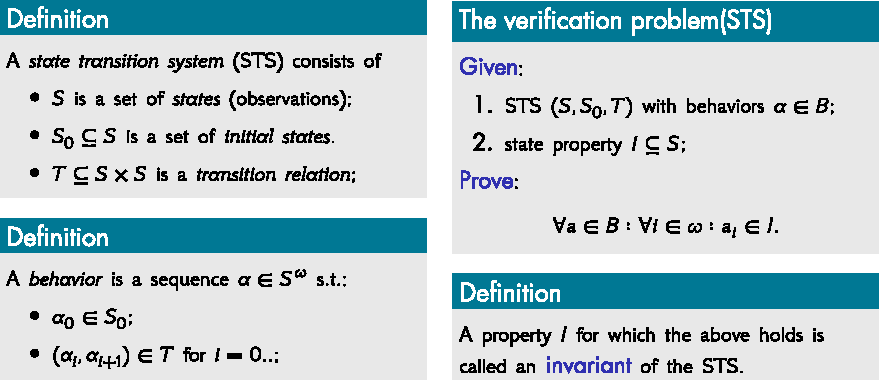
\includegraphics[width=\unitlength,page=1]{Figures/L7_sts.pdf}}%
  \end{picture}%
\endgroup%
    
\end{minipage}

\paragraph{Invariants: } 
\begin{itemize}
    \item {\textbf{Invariant:}} definition in image above. 
    \item proving invariants is too difficult, thats why we need inductive invariants.
    \item \textbf{Inductive Invariants:} An inductive invariant of a STS is a state property I such that \textcolor{blue}{$S_0 \subseteq I$ and $T[I] \subseteq I$}.
    \item \textbf{Theorem: } Every inductive invariant is an invariant.
\end{itemize}

\paragraph{How to prove inductiveness automatically?} 
\begin{itemize}
    \item Use the \textcolor{orange}{strongest postcondition} operator \textbf{sp} : Program x Assertion $\rightarrow$ Assertion.
\end{itemize}{}

\begin{minipage}{0.9\linewidth}
    \centering      
    \def\svgwidth{\linewidth}
    %% Creator: Inkscape inkscape 0.92.4, www.inkscape.org
%% PDF/EPS/PS + LaTeX output extension by Johan Engelen, 2010
%% Accompanies image file 'L7_strongest_postcondition.pdf' (pdf, eps, ps)
%%
%% To include the image in your LaTeX document, write
%%   \input{<filename>.pdf_tex}
%%  instead of
%%   \includegraphics{<filename>.pdf}
%% To scale the image, write
%%   \def\svgwidth{<desired width>}
%%   \input{<filename>.pdf_tex}
%%  instead of
%%   \includegraphics[width=<desired width>]{<filename>.pdf}
%%
%% Images with a different path to the parent latex file can
%% be accessed with the `import' package (which may need to be
%% installed) using
%%   \usepackage{import}
%% in the preamble, and then including the image with
%%   \import{<path to file>}{<filename>.pdf_tex}
%% Alternatively, one can specify
%%   \graphicspath{{<path to file>/}}
%% 
%% For more information, please see info/svg-inkscape on CTAN:
%%   http://tug.ctan.org/tex-archive/info/svg-inkscape
%%
\begingroup%
  \makeatletter%
  \providecommand\color[2][]{%
    \errmessage{(Inkscape) Color is used for the text in Inkscape, but the package 'color.sty' is not loaded}%
    \renewcommand\color[2][]{}%
  }%
  \providecommand\transparent[1]{%
    \errmessage{(Inkscape) Transparency is used (non-zero) for the text in Inkscape, but the package 'transparent.sty' is not loaded}%
    \renewcommand\transparent[1]{}%
  }%
  \providecommand\rotatebox[2]{#2}%
  \newcommand*\fsize{\dimexpr\f@size pt\relax}%
  \newcommand*\lineheight[1]{\fontsize{\fsize}{#1\fsize}\selectfont}%
  \ifx\svgwidth\undefined%
    \setlength{\unitlength}{403.18360772bp}%
    \ifx\svgscale\undefined%
      \relax%
    \else%
      \setlength{\unitlength}{\unitlength * \real{\svgscale}}%
    \fi%
  \else%
    \setlength{\unitlength}{\svgwidth}%
  \fi%
  \global\let\svgwidth\undefined%
  \global\let\svgscale\undefined%
  \makeatother%
  \begin{picture}(1,0.25458509)%
    \lineheight{1}%
    \setlength\tabcolsep{0pt}%
    \put(0,0){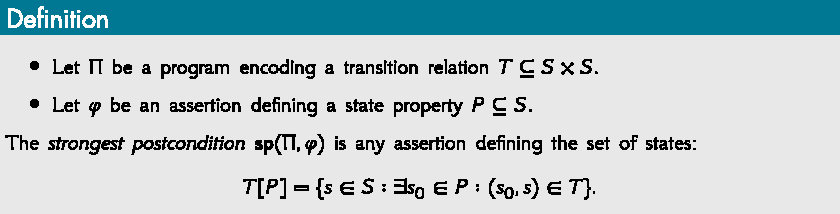
\includegraphics[width=\unitlength,page=1]{Figures/L7_strongest_postcondition.pdf}}%
  \end{picture}%
\endgroup%
    
\end{minipage}
\\

\begin{enumerate}
    \item 
    \begin{itemize}
        \item [a)] A state transition system ($S$, $S_0$, $T$) is given by two progtams \texttt{init} and \texttt{step}:
        \item[] \texttt{init; \textbf{while true} \{ step; \}}
        \item [b)] A candidate invariant / is given by a formula $\varphi$.
    \end{itemize}
    \item Use and automated theorem prover to prove the validity of the formulas:
    \begin{itemize}
        \item[a)] $\textbf{sp}$ (\texttt{init, true}) $\rightarrow$ $\varphi$; (encodes $S_0 \subseteq I$)
        \item[b)] $\textbf{sp}$ (\texttt{step,}) $\varphi \rightarrow \varphi$; (encodes $T[I] \subseteq I$)
    \end{itemize}{}
    \item[$\rightarrow$] \textcolor{blue}{Example of this process on slide 15.}
\end{enumerate}

\paragraph{Computing  $sp(\Pi,\varphi)$}\textbf{by symbolic execution:}

\begin{minipage}{0.9\linewidth}
    \centering      
    \def\svgwidth{\linewidth}
    %% Creator: Inkscape inkscape 0.92.4, www.inkscape.org
%% PDF/EPS/PS + LaTeX output extension by Johan Engelen, 2010
%% Accompanies image file 'L7_symbolic_exec.pdf' (pdf, eps, ps)
%%
%% To include the image in your LaTeX document, write
%%   \input{<filename>.pdf_tex}
%%  instead of
%%   \includegraphics{<filename>.pdf}
%% To scale the image, write
%%   \def\svgwidth{<desired width>}
%%   \input{<filename>.pdf_tex}
%%  instead of
%%   \includegraphics[width=<desired width>]{<filename>.pdf}
%%
%% Images with a different path to the parent latex file can
%% be accessed with the `import' package (which may need to be
%% installed) using
%%   \usepackage{import}
%% in the preamble, and then including the image with
%%   \import{<path to file>}{<filename>.pdf_tex}
%% Alternatively, one can specify
%%   \graphicspath{{<path to file>/}}
%% 
%% For more information, please see info/svg-inkscape on CTAN:
%%   http://tug.ctan.org/tex-archive/info/svg-inkscape
%%
\begingroup%
  \makeatletter%
  \providecommand\color[2][]{%
    \errmessage{(Inkscape) Color is used for the text in Inkscape, but the package 'color.sty' is not loaded}%
    \renewcommand\color[2][]{}%
  }%
  \providecommand\transparent[1]{%
    \errmessage{(Inkscape) Transparency is used (non-zero) for the text in Inkscape, but the package 'transparent.sty' is not loaded}%
    \renewcommand\transparent[1]{}%
  }%
  \providecommand\rotatebox[2]{#2}%
  \newcommand*\fsize{\dimexpr\f@size pt\relax}%
  \newcommand*\lineheight[1]{\fontsize{\fsize}{#1\fsize}\selectfont}%
  \ifx\svgwidth\undefined%
    \setlength{\unitlength}{414.1536245bp}%
    \ifx\svgscale\undefined%
      \relax%
    \else%
      \setlength{\unitlength}{\unitlength * \real{\svgscale}}%
    \fi%
  \else%
    \setlength{\unitlength}{\svgwidth}%
  \fi%
  \global\let\svgwidth\undefined%
  \global\let\svgscale\undefined%
  \makeatother%
  \begin{picture}(1,0.44668589)%
    \lineheight{1}%
    \setlength\tabcolsep{0pt}%
    \put(0,0){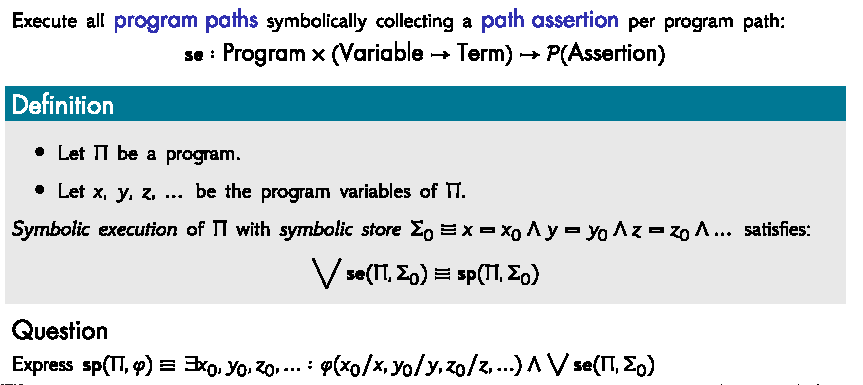
\includegraphics[width=\unitlength,page=1]{Figures/L7_symbolic_exec.pdf}}%
  \end{picture}%
\endgroup%
    
\end{minipage}

\begin{itemize}
    \item If $\Pi$ contains loops then, \#paths = $\infty$, requiring more sophisticated techniques.
    \item [$\rightarrow$] \textcolor{blue}{Example of this process on slide 18.}
\end{itemize}{}

\paragraph{How to prove non-inductive variants?}
\begin{itemize}
    \item Find an inductive strengthening $l$ manually: $l$ is inductive and $l \rightarrow \varphi$.
    \item and prove analogously the strengthening $l$ automatically.
\end{itemize}{}




